\documentclass[../main.tex]{subfiles}

\begin{document}
    \subsection{Runtime}
    Runtimes which are reported here in second are average of total execution time for first and second run.\\
    Almost in all queries Postgres took much more time to generating results (except fot query21). For Q17 and Q20, Postgres was ran for 5 days but no results were achieved so the process was killed.\\
    \begin{minipage}{\textwidth}
        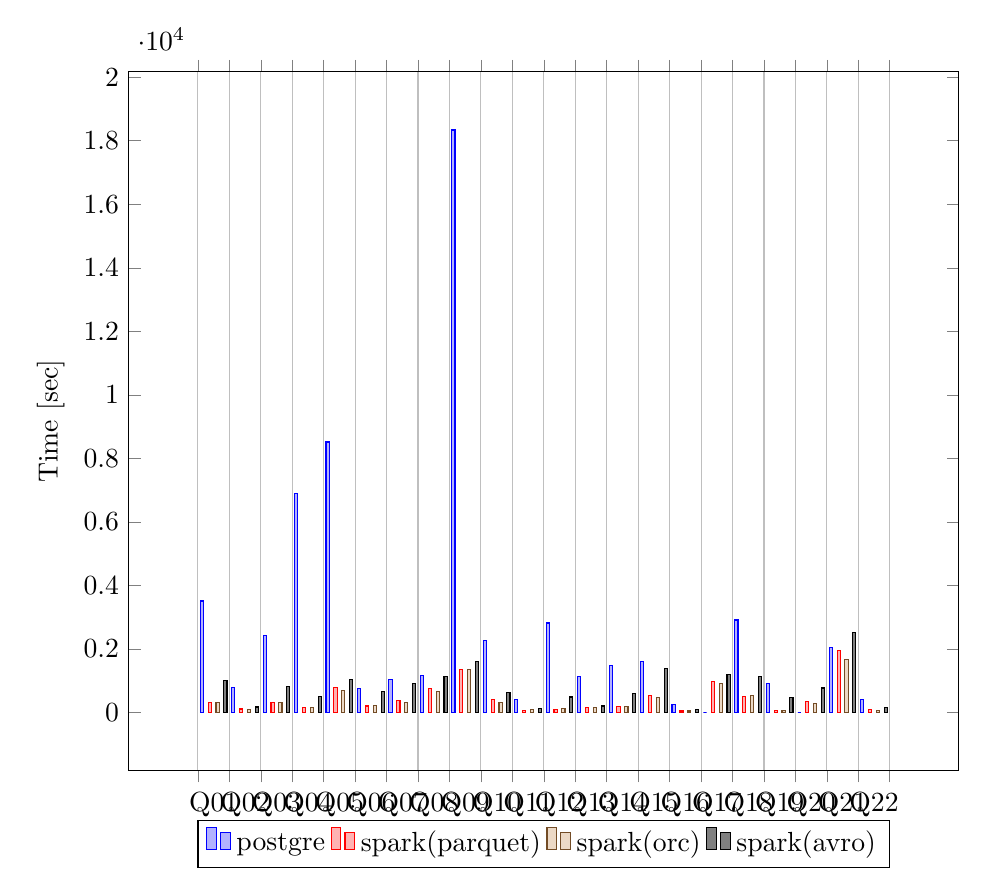
\begin{tikzpicture}
            \begin{axis}[
                ybar,
                width=\textwidth,
                ybar interval=0.4,
                legend style={at={(0.5,-0.07)},
                anchor=north,legend columns=-1},
                ylabel={Time [sec]},
                symbolic x coords={Q01,Q02,Q03,Q04,Q05,Q06,Q07,Q08,Q09,Q10,Q11,Q12,Q13,Q14,Q15,Q16,Q17,Q18,Q19,Q20,Q21,Q22,dummy},
                ]
                \addplot coordinates { (Q01,3508) (Q02,787) (Q03,2429) (Q04,6888) (Q05,8516) (Q06,744) (Q07,1042) (Q08,1156) (Q09,18340) (Q10,2263) (Q11,404) (Q12,2817) (Q13,1125) (Q14,1491) (Q15,1592) (Q16,257) (Q17,0) (Q18,2909) (Q19,907) (Q20,0) (Q21,2042) (Q22,414) (dummy,0) };
                \addplot coordinates { (Q01,304) (Q02,109) (Q03,312) (Q04,145) (Q05,796) (Q06,201) (Q07,373) (Q08,748) (Q09,1353) (Q10,413) (Q11,72) (Q12,104) (Q13,162) (Q14,196) (Q15,523) (Q16,46) (Q17,987) (Q18,495) (Q19,69) (Q20,342) (Q21,1945) (Q22,79) (dummy,0) };
                \addplot coordinates { (Q01,310) (Q02, 91) (Q03, 311) (Q04, 148) (Q05, 677) (Q06, 210) (Q07, 314) (Q08, 655) (Q09, 1349) (Q10, 301) (Q11, 79) (Q12, 135) (Q13, 157) (Q14, 196) (Q15, 463) (Q16, 46) (Q17, 915) (Q18, 524) (Q19, 57) (Q20, 293) (Q21, 1671) (Q22,73) (dummy,0) };
                \addplot coordinates { (Q01,1001) (Q02, 171) (Q03, 811) (Q04, 514) (Q05, 1035) (Q06, 655) (Q07, 897) (Q08, 1130) (Q09, 1616) (Q10, 619) (Q11, 117) (Q12, 485) (Q13, 201) (Q14, 610) (Q15, 1390) (Q16, 99) (Q17, 1199) (Q18, 1129) (Q19, 469) (Q20, 768) (Q21, 2525) (Q22,145) (dummy,0) };
                \legend{postgre, spark(parquet), spark(orc), spark(avro)}
            \end{axis}
        \end{tikzpicture}
    \end{minipage}

    \begin{minipage}{\textwidth}
        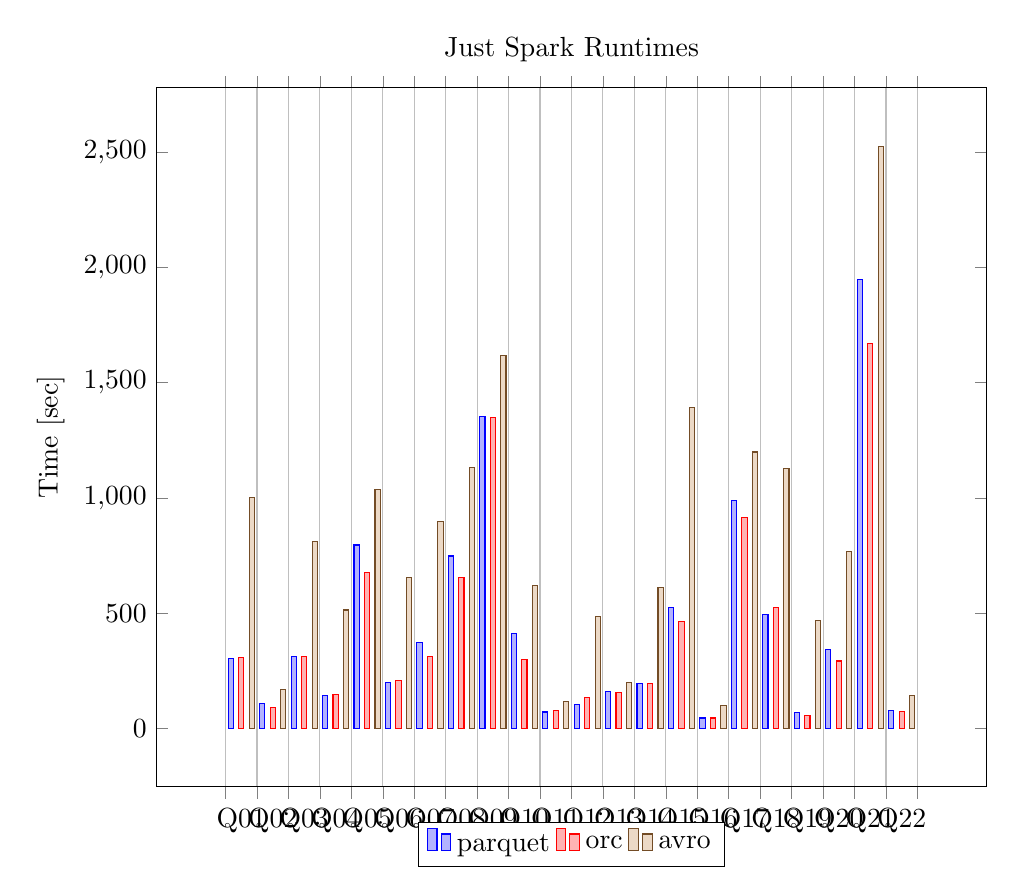
\begin{tikzpicture}
            \begin{axis}[
                ybar,
                title={Just Spark Runtimes},
                width=\textwidth,
                ybar interval=0.5,
                legend style={at={(0.5,-0.05)},
                anchor=north,legend columns=-1},
                ylabel={Time [sec]},
                symbolic x coords={Q01,Q02,Q03,Q04,Q05,Q06,Q07,Q08,Q09,Q10,Q11,Q12,Q13,Q14,Q15,Q16,Q17,Q18,Q19,Q20,Q21,Q22,dummy},
                xtick=data,
                % nodes near coords,
                nodes near coords align={vertical},
                ]
                \addplot coordinates { (Q01,304) (Q02,109) (Q03,312) (Q04,145) (Q05,796) (Q06,201) (Q07,373) (Q08,748) (Q09,1353) (Q10,413) (Q11,72) (Q12,104) (Q13,162) (Q14,196) (Q15,523) (Q16,46) (Q17,987) (Q18,495) (Q19,69) (Q20,342) (Q21,1945) (Q22,79) (dummy,0)};
                \addplot coordinates { (Q01, 310) (Q02, 91) (Q03, 311) (Q04, 148) (Q05, 677) (Q06, 210) (Q07, 314) (Q08, 655) (Q09, 1349) (Q10, 301) (Q11, 79) (Q12, 135) (Q13, 157) (Q14, 196) (Q15, 463) (Q16, 46) (Q17, 915) (Q18, 524) (Q19, 57) (Q20, 293) (Q21, 1671) (Q22, 73) (dummy,0)};
                \addplot coordinates { (Q01, 1001) (Q02, 171) (Q03, 811) (Q04, 514) (Q05, 1035) (Q06, 655) (Q07, 897) (Q08, 1130) (Q09, 1616) (Q10, 619) (Q11, 117) (Q12, 485) (Q13, 201) (Q14, 610) (Q15, 1390) (Q16, 99) (Q17, 1199) (Q18, 1129) (Q19, 469) (Q20, 768) (Q21, 2525) (Q22, 145) (dummy,0)};
                \legend{parquet, orc, avro}
            \end{axis}
        \end{tikzpicture}
    \end{minipage}
    As plot shows, every test on avro FS took more time to process. Also except for Q06 all parquet test rans longer than orc.
    \begin{table}
        \begin{center}
            \begin{tabular}{ |c|c|c|c|c| } 
            \hline
            Query num & postgre & spark(parquet) & spark(orc) & spark(avro)\\
            \hline
            Q01 & 3508 & 304 & 310 & 1001\\
            Q02 & 787 & 109 & 91 & 171\\
            Q03 & 2429 & 312 & 311 & 811\\
            Q04 & 6888 & 145 & 148 & 514\\
            Q05 & 8516 & 796 & 677 & 1035\\
            Q06 & 744 & 201 & 210 & 655\\
            Q07 & 1042 & 373 & 314 & 897\\
            Q08 & 1156 & 748 & 655 & 1130\\
            Q09 & 18340 & 1353 & 1349 & 1616\\
            Q10 & 2263 & 413 & 301 & 619\\
            Q11 & 404 & 72 & 79 & 117\\
            Q12 & 2817 & 104 & 135 & 485\\
            Q13 & 1125 & 162 & 157 & 201\\
            Q14 & 1491 & 196 & 196 & 610\\
            Q15 & 1592 & 523 & 463 & 1390\\
            Q16 & 257 & 46 & 46 & 99\\
            Q17 & more than 546734 & 987 & 915 & 1199\\
            Q18 & 2909 & 495 & 524 & 1129\\
            Q19 & 907 & 69 & 57 & 469\\
            Q20 & more than 522760 & 342 & 293 & 768\\
            Q21 & 2042 & 1945 & 1671 & 2525\\
            Q22 & 414 & 79 & 73 & 145\\
            \hline
            \end{tabular}
            \\[1pt]
            \caption{Runtimes in seconds}
        \end{center}
    \end{table}

    \subsection{Load}
    Load average for spark with parquet is higher than others and postgres has minimum load average.(maybe because it took longer than other tests). comparing orc tests and Avro tests doesnt get us concret result. Their load average are close together and sometime avro is higher and sometime vice versa.\\
    \begin{minipage}{\textwidth}
        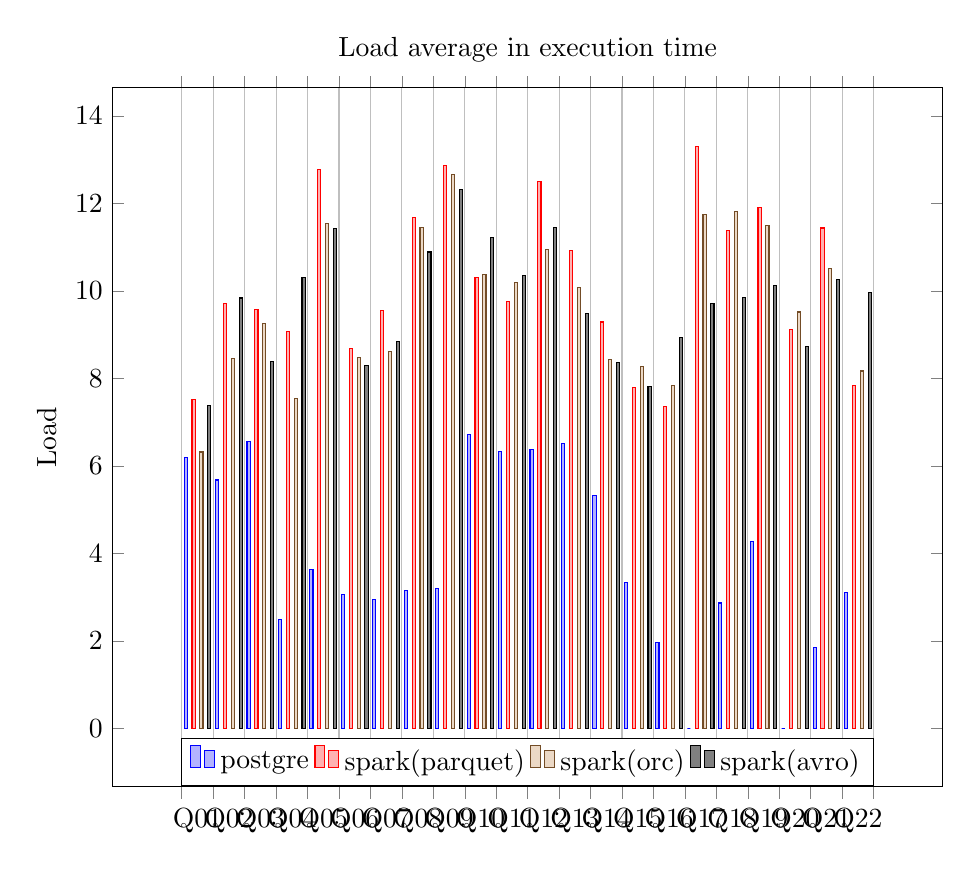
\begin{tikzpicture}
            \begin{axis}[
                ybar,
                width=\textwidth,
                ybar interval=0.4,
                title={Load average in execution time},
                legend style={at={(0.5,0.07)},
                anchor=north,legend columns=-1},
                ylabel={Load},
                symbolic x coords={Q01,Q02,Q03,Q04,Q05,Q06,Q07,Q08,Q09,Q10,Q11,Q12,Q13,Q14,Q15,Q16,Q17,Q18,Q19,Q20,Q21,Q22,dummy},
                ]
                \addplot coordinates { (Q01,6.20) (Q02,5.68) (Q03,6.57) (Q04,2.50) (Q05,3.64) (Q06,3.06) (Q07,2.95) (Q08,3.16) (Q09,3.21) (Q10,6.71) (Q11,6.33) (Q12,6.38) (Q13,6.51) (Q14,5.32) (Q15,3.33) (Q16,1.96) (Q17,0) (Q18,2.87) (Q19,4.27) (Q20,0) (Q21,1.86) (Q22,3.10) (dummy,0) };
                \addplot coordinates { (Q01,7.51) (Q02,9.71) (Q03,9.57) (Q04,9.07) (Q05,12.78) (Q06,8.68) (Q07,9.55) (Q08,11.68) (Q09,12.86) (Q10,10.31) (Q11,9.76) (Q12,12.50) (Q13,10.92) (Q14,9.29) (Q15,7.79) (Q16,7.36) (Q17,13.31) (Q18,11.38) (Q19,11.90) (Q20,9.11) (Q21,11.44) (Q22,7.84) (dummy,0) };
                \addplot coordinates { (Q01,6.32) (Q02,8.46) (Q03,9.26) (Q04,7.55) (Q05,11.55) (Q06,8.47) (Q07,8.61) (Q08,11.46) (Q09,12.66) (Q10,10.38) (Q11,10.20) (Q12,10.94) (Q13,10.08) (Q14,8.43) (Q15,8.27) (Q16,7.83) (Q17,11.74) (Q18,11.82) (Q19,11.49) (Q20,9.52) (Q21,10.51) (Q22,8.17) (dummy,0) };
                \addplot coordinates { (Q01,7.39) (Q02,9.84) (Q03,8.39) (Q04,10.30) (Q05,11.42) (Q06,8.29) (Q07,8.84) (Q08,10.89) (Q09,12.32) (Q10,11.22) (Q11,10.36) (Q12,11.46) (Q13,9.49) (Q14,8.36) (Q15,7.81) (Q16,8.94) (Q17,9.71) (Q18,9.86) (Q19,10.13) (Q20,8.74) (Q21,10.26) (Q22,9.97) (dummy,0) };
                \legend{postgre, spark(parquet), spark(orc), spark(avro)}
            \end{axis}
        \end{tikzpicture}
    \end{minipage}
    \begin{table}
        \begin{center}
            \begin{tabular}{ |c|c|c|c|c| } 
            \hline
            Query num & postgre & spark(avro) & spark(orc) & spark(parquet) \\
            \hline
            Q01 & 6.20 & 7.39 & 6.32 & 7.51 \\
            Q02 & 5.68 & 9.84 & 8.46 & 9.71 \\
            Q03 & 6.57 & 8.39 & 9.26 & 9.57 \\
            Q04 & 2.50 & 10.30 & 7.55 & 9.07 \\
            Q05 & 3.64 & 11.42 & 11.55 & 12.78 \\
            Q06 & 3.06 & 8.29 & 8.47 & 8.68 \\
            Q07 & 2.95 & 8.84 & 8.61 & 9.55 \\
            Q08 & 3.16 & 10.89 & 11.46 & 11.68 \\
            Q09 & 3.21 & 12.32 & 12.66 & 12.86 \\
            Q10 & 6.71 & 11.22 & 10.38 & 10.31 \\
            Q11 & 6.33 & 10.36 & 10.20 & 9.76 \\
            Q12 & 6.38 & 11.46 & 10.94 & 12.50 \\
            Q13 & 6.51 & 9.49 & 10.08 & 10.92 \\
            Q14 & 5.32 & 8.36 & 8.43 & 9.29 \\
            Q15 & 3.33 & 7.81 & 8.27 & 7.79 \\
            Q16 & 1.96 & 8.94 & 7.83 & 7.36 \\
            Q17 & - & 9.71 & 11.74 & 13.31 \\
            Q18 & 2.87 & 9.86 & 11.82 & 11.38 \\
            Q19 & 4.27 & 10.13 & 11.49 & 11.90 \\
            Q20 & - & 8.74 & 9.52 & 9.11 \\
            Q21 & 1.86 & 10.26 & 10.51 & 11.44 \\
            Q22 & 3.10 & 9.97 & 8.17 & 7.84 \\
            \hline
            \end{tabular}
            \\[1pt]
            \caption{Runtimes in seconds}
        \end{center}
    \end{table}

    \subsection{Average Disk Usage}
    Unlike other parameters overall disk usage of postgres is higher the other in spite of long runtime. This is because postgres tries to persist everything on disk and correspond to join implementation in postgres DBMS (except the Q09, because Q09 takes too much time). Between spark tests avro has higher disk usage in spite of long runtime. According to queries disk usage plots, Spark reads  file in format of avro more time than the other formats. Overall disk usage of parquet is slightly higher than orc.
    For orc tests, it seemed too much writing  on disk is bottleneck. Unlike parquet and avro , it uses disk Almost just for reading, even after free memory reading from disk continues to load needed data.\\
    \begin{minipage}{\textwidth}
        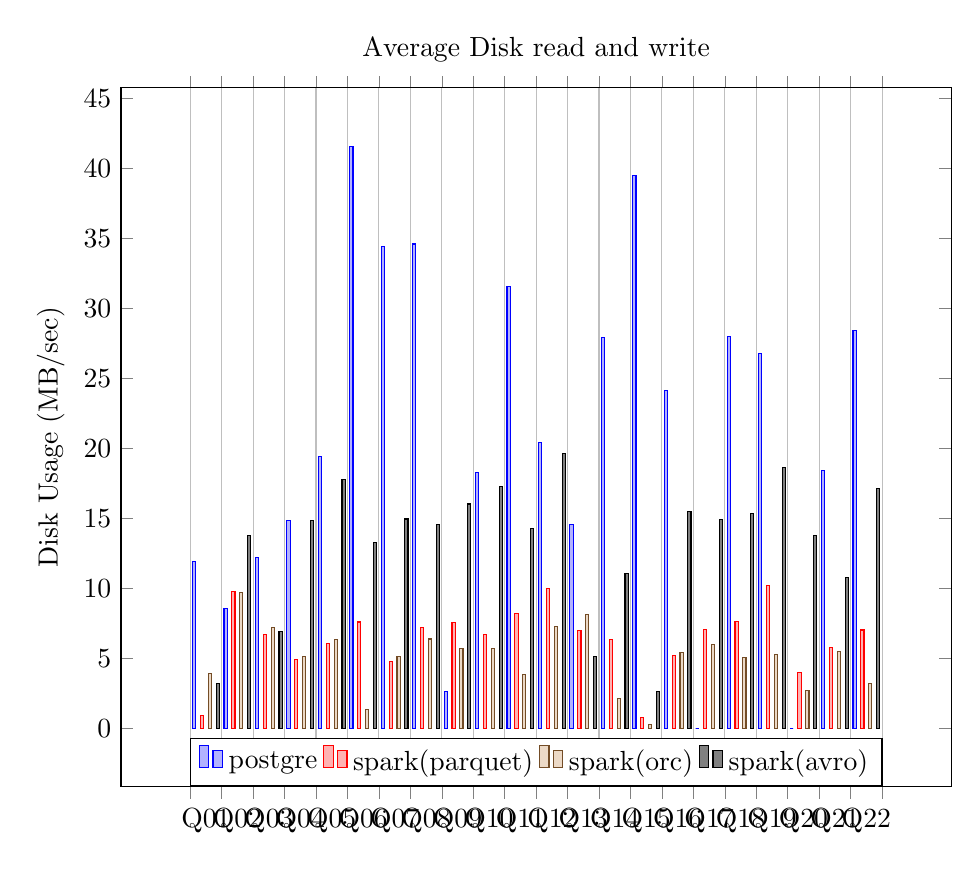
\begin{tikzpicture}
            \begin{axis}[
                ybar,
                width=\textwidth,
                ybar interval=0.4,
                title={Average Disk read and write},
                legend style={at={(0.5,0.07)},
                anchor=north,legend columns=-1},
                ylabel={Disk Usage (MB/sec)},
                symbolic x coords={Q01,Q02,Q03,Q04,Q05,Q06,Q07,Q08,Q09,Q10,Q11,Q12,Q13,Q14,Q15,Q16,Q17,Q18,Q19,Q20,Q21,Q22,dummy},
                ]
                \addplot coordinates { (Q01,11.96) (Q02,8.56) (Q03,12.19) (Q04,14.88) (Q05,19.41) (Q06,41.61) (Q07,34.43) (Q08,34.62) (Q09,2.64) (Q10,18.28) (Q11,31.56) (Q12,20.44) (Q13,14.61) (Q14,27.92) (Q15,39.52) (Q16,24.12) (Q17,0) (Q18,27.98) (Q19,26.78) (Q20,0) (Q21,18.45) (Q22,28.41) (dummy,0) };
                \addplot coordinates { (Q01,0.91) (Q02,9.80) (Q03,6.70) (Q04,4.93) (Q05,6.06) (Q06,7.61) (Q07,4.80) (Q08,7.19) (Q09,7.57) (Q10,6.70) (Q11,8.21) (Q12,10.01) (Q13,7.01) (Q14,6.35) (Q15,0.79) (Q16,5.20) (Q17,7.09) (Q18,7.64) (Q19,10.22) (Q20,4.00) (Q21,5.78) (Q22,7.04) (dummy,0) };
                \addplot coordinates { (Q01,3.92) (Q02,9.70) (Q03,7.23) (Q04,5.15) (Q05,6.37) (Q06,1.36) (Q07,5.18) (Q08,6.40) (Q09,5.74) (Q10,5.74) (Q11,3.87) (Q12,7.27) (Q13,8.16) (Q14,2.17) (Q15,0.31) (Q16,5.46) (Q17,6.00) (Q18,5.10) (Q19,5.30) (Q20,2.71) (Q21,5.52) (Q22,3.23) (dummy,0) };
                \addplot coordinates { (Q01,3.23) (Q02,13.78) (Q03,6.91) (Q04,14.88) (Q05,17.81) (Q06,13.30) (Q07,14.97) (Q08,14.59) (Q09,16.04) (Q10,17.30) (Q11,14.29) (Q12,19.67) (Q13,5.13) (Q14,11.06) (Q15,2.63) (Q16,15.50) (Q17,14.94) (Q18,15.39) (Q19,18.64) (Q20,13.77) (Q21,10.81) (Q22,17.12) (dummy,0) };
                \legend{postgre, spark(parquet), spark(orc), spark(avro)}
            \end{axis}
        \end{tikzpicture}
    \end{minipage}
    \begin{table}
        \begin{center}
            \begin{tabular}{ |c|c|c|c|c| } 
            \hline
            Query num & postgre & spark(avro) & spark(orc) & spark(parquet) \\
            \hline
            Q01 & 11.96 & 3.23 & 3.92 & 0.91 \\
            Q02 & 8.56 & 13.78 & 9.70 & 9.80 \\
            Q03 & 12.19 & 6.91 & 7.23 & 6.70 \\
            Q04 & 14.88 & 14.88 & 5.15 & 4.93 \\
            Q05 & 19.41 & 17.81 & 6.37 & 6.06 \\
            Q06 & 41.61 & 13.30 & 1.36 & 7.61 \\
            Q07 & 34.43 & 14.97 & 5.18 & 4.80 \\
            Q08 & 34.62 & 14.59 & 6.40 & 7.19 \\
            Q09 & 2.64 & 16.04 & 5.74 & 7.57 \\
            Q10 & 18.28 & 17.30 & 5.74 & 6.70 \\
            Q11 & 31.56 & 14.29 & 3.87 & 8.21 \\
            Q12 & 20.44 & 19.67 & 7.27 & 10.01 \\
            Q13 & 14.61 & 5.13 & 8.16 & 7.01 \\
            Q14 & 27.92 & 11.06 & 2.17 & 6.35 \\
            Q15 & 39.52 & 2.63 & 0.31 & 0.79 \\
            Q16 & 24.12 & 15.50 & 5.46 & 5.20 \\
            Q17 & - & 14.94 & 6.00 & 7.09 \\
            Q18 & 27.98 & 15.39 & 5.10 & 7.64 \\
            Q19 & 26.78 & 18.64 & 5.30 & 10.22 \\
            Q20 & - & 13.77 & 2.71 & 4.00 \\
            Q21 & 18.45 & 10.81 & 5.52 & 5.78 \\
            Q22 & 28.41 & 17.12 & 3.23 & 7.04 \\
            \hline
            \end{tabular}
            \\[1pt]
            \caption{Average disk read and write (MB/sec)}
        \end{center}
    \end{table}

    \subsection{Memory}
    Memory average results are so close together that we cant make certain results. Except for orc format which seems use less memory than the others in some queries.\\ 
    In all sparks tests with diffrent file formats no obvious diffrence can be seen. Just amount of reading from disk and freeing memory is variant among tests.\\
    Overally spark uses memory much better than postgres and most effective parameter on spark function is reading less from disk. which avro makes it better than other file systems.\\    
    It seemed spark with avro free memory and load data more time than other spark runs.\\
    % \pagebreak
    \begin{minipage}[t]{\textwidth}
        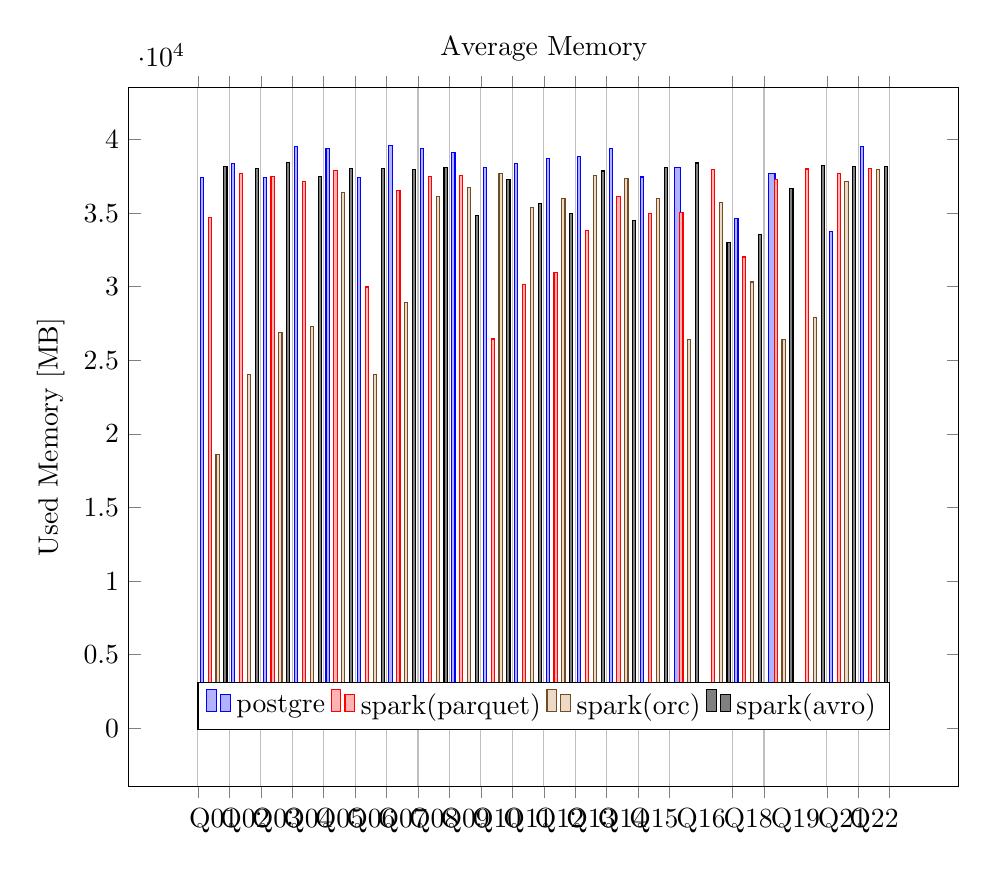
\begin{tikzpicture}
            \begin{axis}[
                ybar,
                width=\textwidth,
                ybar interval=0.4,
                title={Average Memory},
                legend style={at={(0.5,0.15)},
                anchor=north,legend columns=-1},
                ylabel={Used Memory [MB]},
                symbolic x coords={Q01,Q02,Q03,Q04,Q05,Q06,Q07,Q08,Q09,Q10,Q11,Q12,Q13,Q14,Q15,Q16,Q17,Q18,Q19,Q20,Q21,Q22,dummy},
                ]
                \addplot coordinates { (Q01,37415.77) (Q02,38404.04) (Q03,37404.01) (Q04,39552.73) (Q05,39370.85) (Q06,37423.94) (Q07,39577.62) (Q08,39370.30) (Q09,39136.33) (Q10,38100.66) (Q11,38399.85) (Q12,38726.13) (Q13,38832.73) (Q14,39395.19) (Q15,37460.35) (Q16,38097.41) (Q18,34627.95) (Q19,37715.97) (Q21,33771.81) (Q22,39518.21) (dummy,0) };
                \addplot coordinates { (Q01,34721.47) (Q02,37669.72) (Q03,37478.01) (Q04,37134.43) (Q05,37925.04) (Q06,29986.37) (Q07,36546.44) (Q08,37520.41) (Q09,37540.41) (Q10,26451.74) (Q11,30161.78) (Q12,30997.83) (Q13,33825.26) (Q14,36162.94) (Q15,35000.78) (Q16,35028.55) (Q17,37951.60) (Q18,32025.87) (Q19,37318.39) (Q20,37999.16) (Q21,37699.89) (Q22,38057.87) (dummy,0) };
                \addplot coordinates { (Q01,18584.58) (Q02,24040.47) (Q03,26894.77) (Q04,27317.29) (Q05,36390.49) (Q06,24064.27) (Q07,28937.86) (Q08,36116.59) (Q09,36729.97) (Q10,37723.28) (Q11,35361.91) (Q12,36023.24) (Q13,37552.20) (Q14,37351.88) (Q15,35972.20) (Q16,26438.05) (Q17,35718.01) (Q18,30325.33) (Q19,26440.09) (Q20,27935.17) (Q21,37143.61) (Q22,37967.55) (dummy,0) };
                \addplot coordinates { (Q01,38187.44) (Q02,38049.24) (Q03,38428.72) (Q04,37495.57) (Q05,38011.38) (Q06,38056.31) (Q07,37942.76) (Q08,38093.10) (Q09,34857.56) (Q10,37285.80) (Q11,35672.18) (Q12,34995.34) (Q13,37867.98) (Q14,34507.11) (Q15,38092.25) (Q16,38406.51) (Q17,33030.43) (Q18,33576.10) (Q19,36706.26) (Q20,38214.14) (Q21,38188.50) (Q22,38164.89) (dummy,0) };
                \legend{postgre, spark(parquet), spark(orc), spark(avro)}
            \end{axis}
        \end{tikzpicture}
    \end{minipage}
    \begin{table}
        \begin{center}
            \begin{tabular}{ |c|c|c|c|c| } 
            \hline
            Query num & postgre & spark(avro) & spark(orc) & spark(parquet) \\
            \hline
            Q01 & 37415.77 & 38187.44 & 18584.58 & 34721.47\\
            Q02 & 38404.04 & 38049.24 & 24040.47 & 37669.72\\
            Q03 & 37404.01 & 38428.72 & 26894.77 & 37478.01\\
            Q04 & 39552.73 & 37495.57 & 27317.29 & 37134.43\\
            Q05 & 39370.85 & 38011.38 & 36390.49 & 37925.04\\
            Q06 & 37423.94 & 38056.31 & 24064.27 & 29986.37\\
            Q07 & 39577.62 & 37942.76 & 28937.86 & 36546.44\\
            Q08 & 39370.30 & 38093.10 & 36116.59 & 37520.41\\
            Q09 & 39136.33 & 34857.56 & 36729.97 & 37540.41\\
            Q10 & 38100.66 & 37285.80 & 37723.28 & 26451.74\\
            Q11 & 38399.85 & 35672.18 & 35361.91 & 30161.78\\
            Q12 & 38726.13 & 34995.34 & 36023.24 & 30997.83\\
            Q13 & 38832.73 & 37867.98 & 37552.20 & 33825.26\\
            Q14 & 39395.19 & 34507.11 & 37351.88 & 36162.94\\
            Q15 & 37460.35 & 38092.25 & 35972.20 & 35000.78\\
            Q16 & 38097.41 & 38406.51 & 26438.05 & 35028.55\\
            Q17 & - & 33030.43 & 35718.01 & 37951.60\\
            Q18 & 34627.95 & 33576.10 & 30325.33 & 32025.87\\
            Q19 & 37715.97 & 36706.26 & 26440.09 & 37318.39\\
            Q20 & - & 38214.14 & 27935.17 & 37999.16\\
            Q21 & 33771.81 & 38188.50 & 37143.61 & 37699.89\\
            Q22 & 39518.21 & 38164.89 & 37967.55 & 38057.87\\
            \hline
            \end{tabular}
            \\[1pt]
            \caption{Average memory usage (MB)}
        \end{center}
    \end{table}
\end{document}
